\documentclass[journal,transmag]{IEEEtran}
\ifCLASSINFOpdf
\else
\fi

\usepackage{amsmath}
\usepackage{subcaption}
\usepackage{graphicx}
\usepackage{url}
\usepackage{array}
\usepackage{algorithm}
\usepackage{algorithmic}
\usepackage{multicol}
\usepackage{float}
\usepackage{tabularx}
\usepackage{booktabs}
\usepackage[percent]{overpic}
\usepackage{tikz}
\usetikzlibrary{arrows.meta,positioning}

\begin{document}
\title{
  \textbf{SmartCam: A Collaborative Multi-Agent SLAM Framework for Autonomous Navigation}
}

\author{\IEEEauthorblockN{ Mehul Goel, Ashley Garcia, Youjia Tong, Chenghao Xiang}
\IEEEauthorblockA{Electrical \& Computer Engineering, Rice University, Houston, TX 77005 USA}
}

\markboth{Spring 2026 ELEC594}
{Shell \MakeLowercase{\textit{et al.}}: SmartCam Module}

\maketitle

\begin{abstract}
\textit{Abstract--}Autonomous vehicle navigation in large-scale urban and indoor environments faces critical challenges from GPS unavailability, cumulative localization errors, and sensor failures that can compromise safety. Current solutions rely heavily on GPS modules or centralized mapping systems that struggle with scalability and robustness. We propose SmartCam, a collaborative SLAM framework in which multiple cars share local submaps at common landmarks to build globally consistent maps. A central Jetson Orin Nano server coordinates vehicle status updates and collision avoidance by dynamically assigning tasks and unexplored areas. The system integrates a sensor-based Automatic Emergency Braking (AEB) layer for fault tolerance, and a YOLOv8n perception pipeline for semantic obstacle avoidance. Through ROS2-based communication over a Tailscale VPN with the Zenoh protocol, SmartCam enables seamless navigation and mapping in challenging, multicast-restricted environments~\cite{Quigley2009}. Initial evaluations indicate more consistent map construction and lower accumulated localization error than single-robot SLAM approaches.
\end{abstract}

\begin{IEEEkeywords}
Autonomous Driving, Computer Vision, Path Planning, Embedded AI, Smart Mobility, Edge Computing.
\end{IEEEkeywords}

\section{Introduction}
The paradigm shift in autonomous mobile robotics from monolithic single-agent systems to decentralized Multi-Agent Systems (MAS) has unlocked unprecedented capabilities in collective environmental perception and operational redundancy. However, realizing robust Simultaneous Localization and Mapping (SLAM) within such frameworks poses significant computational challenges, particularly when deployed on resource-constrained edge devices \cite{Cadena2016}. The primary bottleneck lies in the high-fidelity processing of asynchronous sensor data, spanning LiDAR point clouds, IMU inertial frames, and visual streams, that must be synthesized in real time to ensure trajectory coherence.

Three fundamental challenges motivate our work. First, GPS is unavailable in many indoor and dense urban environments. Second, odometric position drift accumulates over time, causing maps to degrade without correction. Third, single-sensor architectures are fragile in the face of sensor failure. Existing solutions, such as Tesla's camera-based AI and Waymo's LiDAR stack, address parts of this problem but require costly hardware and do not generalize well to low-cost multi-agent deployments~\cite{Fox1997}.

Our research, titled "SmartCam,'' addresses these challenges through a heterogeneous computing architecture designed to optimize power-to-performance efficiency. By bifurcating the computational workload, we leverage the NVIDIA Jetson Nano for high-level, GPU-accelerated perception—specifically YOLOv8 for real-time object detection—while delegating low-latency sensor fusion and PID-based control loops to the Raspberry Pi 5. This hierarchical design, as seen in Figure 1, enables concurrent execution of deep learning models and high-frequency SLAM optimizations on the HiWonder mobile platform without compromising system stability.

\begin{figure}[t]
\centering
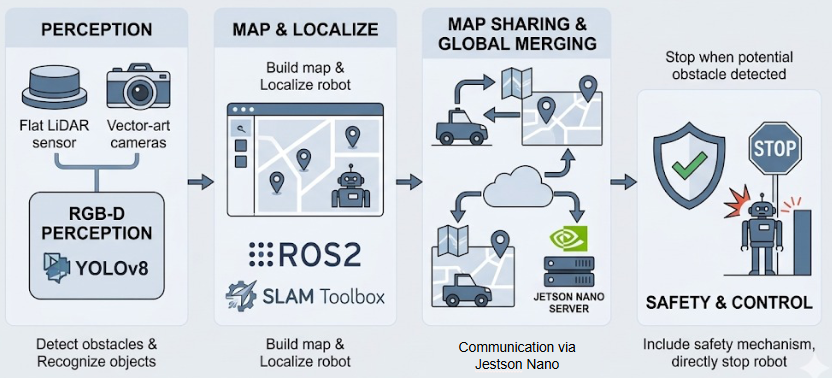
\includegraphics[width=0.48\textwidth]{system_pipeline.png}
\caption{Overall SmartCam system pipeline: sensor perception feeds into ROS2-based SLAM, which streams compressed pose-graphs to a central Jetson Nano server for global map merging and fleet-wide path planning.}
\label{fig:pipeline}
\end{figure}

\section{Methodology}

\subsection{SLAM Toolbox and Multi-Agent Map Merging} For the multi-agent deployment of the SmartCam fleet across the Rice University campus, a centralized 2D map-merging architecture was selected to balance edge-compute constraints with robust navigation capabilities. To overcome the strict NAT and multicast restrictions in the university's wireless infrastructure, the communication pipeline uses a Tailscale virtual private network and the Zenoh protocol. This architecture ensures secure, low-latency, unicast data transfer between the peripheral rover units (equipped with Raspberry Pi 4s) and the central mapping server (hosted on a Jetson Orin Nano). 

Rather than saturating network bandwidth with dense 3D point clouds, each edge unit performs local simultaneous localization and mapping (SLAM) to generate highly compressed 2D occupancy grids and serialized pose graphs. These localized map fragments and odometry constraints are continuously transmitted to the central server. Drawing on graph-based SLAM backend optimization principles, the central server analyzes the incoming data to identify geometric overlaps and inter-robot loop closures. Upon detecting a confident match between two distinct local maps, the server establishes virtual constraints between their respective nodes. A nonlinear least-squares optimizer (GTSAM) is then applied to the newly combined pose graph, elastically deforming and aligning the independent trajectories into a single, unified global coordinate frame. This globally consistent 2D occupancy grid is subsequently broadcast to the individual SmartCam units, providing the necessary environmental context for autonomous, decentralized path planning across the campus.

\begin{figure}[t]
\centering
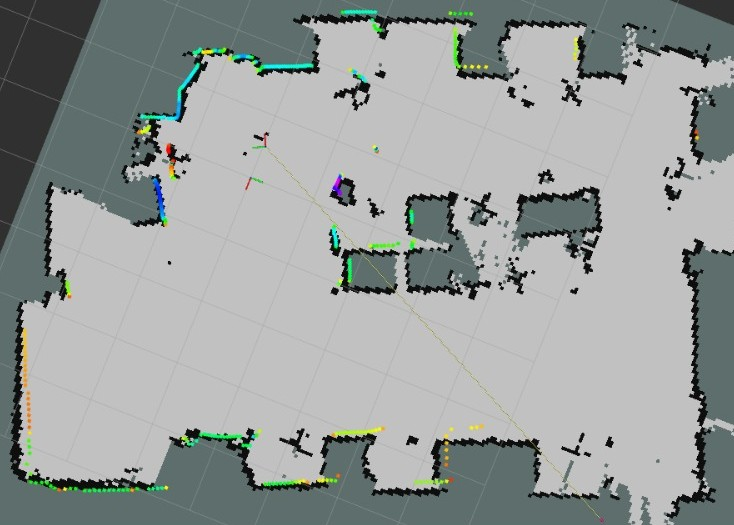
\includegraphics[width=0.4\textwidth]{lidar.jpeg}
\caption{Pose Graph SLAM map using LiDAR}
\label{fig:SLAM1}
\end{figure}

\begin{figure}[t]
\centering
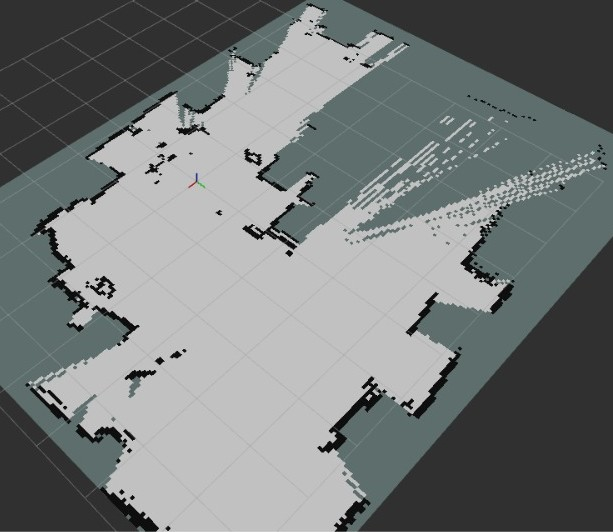
\includegraphics[width=0.4\textwidth]{lidar_encoder.jpeg}
\caption{Large-scale Pose Graph SLAM map visualization.}
\label{fig:SLAM_large}
\end{figure}

\subsection{Sensor Fusion Pipeline and Odometry Calibration} To mitigate the inherent challenges of odometric drift, the data pipeline feeds raw telemetry from HiWonder's LiDAR, depth camera, IMU, and wheel encoders to Toolbox's internal GTSAM-based pose graph optimizer. A primary focus of this implementation is the development of a Kalman filter to fuse wheel encoder data with IMU measurements. This specifically allows tuning of the covariance matrices, thereby ensuring that the IMU compensates for encoder noise and reduces rotation drift. 

This modular approach specifically allows for the sequential integration of sensors, starting with a LiDAR baseline and incrementally adding encoders, IMU, and depth landmarks to better quantify the marginal accuracy gains of each modality. The validation of the sensor fusion layers will be conducted through a comparative analysis of four distinct configurations: LiDAR-only, LiDAR+Encoders, LiDAR+Encoders+IMU, and a full-stack integration including depth-camera landmarks. The end goal will therefore be to quantify these results by comparing the robot's estimated trajectory against a physical ground-truth path using the Root Mean Square Error (RMSE).

\subsection{YOLOv8n Object Detection and Semantic Avoidance} To achieve semantic obstacle avoidance in real-time within the computational constraints of the embedded hardware architecture, as shown in Figure 2, the YOLOv8n (Nano) convolutional neural network was integrated into the primary vision pipeline. The model was aggressively optimized for FP16 precision in TensorRT to maximize inference throughput on the edge GPU, ensuring low-latency detection of dynamic obstacles, such as pedestrians and campus infrastructure. The network processes continuous RGB video streams, regressing bounding box coordinates, and extracting object classification probabilities. 

To transition from 2D pixel space to actionable 3D navigational space, the spatial centroids and boundaries of the detected bounding boxes are correlated with the time-synchronized depth map, enabling the system to extract the median spatial distance to the target. Upon localized detection, the semantic vision node transforms these coordinates from the camera's frame to the rover's base link and dynamically injects the data into the ROS 2 local costmap. By representing classified objects as lethal inflation zones within the costmap, the primary path-planning algorithm is forced to autonomously recalculate its local trajectory, generating smooth, evasive velocity commands to navigate around the identified hazards while maintaining progress toward the global objective \cite{Fox1997}.

\subsection{Automatic Emergency Braking (AEB)} To ensure the physical safety of the autonomous platform and its surrounding environment, an Automatic Emergency Braking (AEB, refer to fig. 5) subsystem was implemented using an HC-SR04 ultrasonic sensor serving as a deterministic, low-latency failsafe independent of the primary visual and LiDAR-based navigation stacks. The methodology relies on acoustic Time-of-Flight (ToF) principles, where a 40 kHz ultrasonic burst is emitted, and the precise duration of the returning echo is measured to calculate the distance to forward obstacles within an operational range of 2cm to 400cm. To mitigate false-positive actuations caused by multipath acoustic reflections or environmental noise, the raw sensor telemetry is conditioned through a real-time median filter before evaluation. 

The Autonomous Emergency Braking (AEB) pipeline is a multi-stage, sequential system designed to detect imminent collisions and trigger an emergency stop using specific components and protocols. It commences when an ultrasonic sensor detects a potential forward obstacle within its effective range. When onboard processing logic (implied at the sensor end or within a dedicated microcontroller immediately interfacing with the sensor before it goes to the primary system, as most simple ultrasonic sensors don't have onboard complex logic and raw data must be processed) determines the obstacle is dangerously close, it directly generates and transmits a critical 'stop message' rather than simple distance data. This message is then instantly sent as a UDP (User Datagram Protocol) packet over a local network connection, bypassing potentially higher-latency layers, and targets a specific port associated with a designated Docker container. Within this container, a receiver service is continuously listening, and upon detecting the incoming stop packet, it extracts the message. Simultaneously, the container hosts a ROS2 (Robot Operating System 2) environment that is actively managing teleoperation. A specific ROS2 node receives the extracted stop information. Recognizing the emergency, this ROS2 node overrides any conflicting teleoperation signals and generates a precise electronic stop signal. This final stop signal is then transmitted from the container's host or dedicated hardware interface to the low-level RRC Lite motor controller. The RRC Lite controller, upon receiving this dedicated instruction, immediately interprets it and actuates the necessary low-level control, cutting power to the motors and potentially applying braking mechanisms, thus bringing the vehicle to an immediate and final halt and preventing a collision.

\begin{figure}[t]
\centering
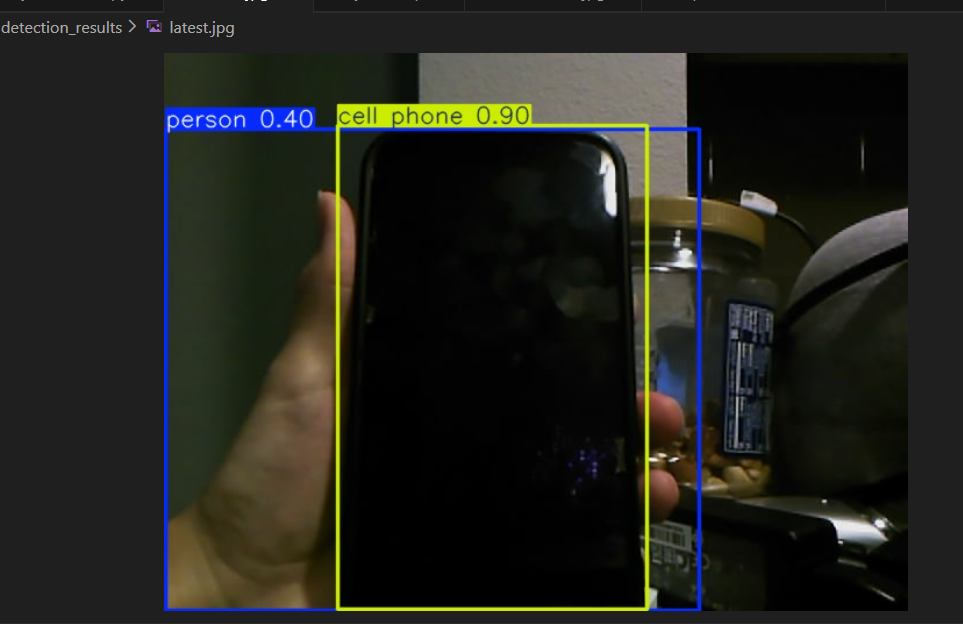
\includegraphics[width=0.45\textwidth]{2.png}
\caption{Object Detection Results: YOLOv8 + Depth Camera}
\label{fig:yolo}
\end{figure}

\subsection{Communication Architecture: Socket to ROS2} Initial prototyping used a tightly coupled point-to-point socket connection between the Jetson Nano and Raspberry Pi. This was replaced by a ROS2 publish-subscribe architecture in which the Jetson publishes detections to a shared ROS2 Topic, and any number of Raspberry Pi subscribers can consume the data, improving scalability and decoupling the perception and control layers. The multi-step pipeline (shown in the multi-layered safety flow) proceeds from obstacle detection, through a UDS socket handoff into a Docker-hosted ROS2 container, through actuation signal generation, and finally to motor stoppage, preserving a clean separation of concerns between the safety layer and the navigation stack.

\subsection{End-to-End Execution Flow}
\textbf{i. Exploration:} Car A and Car B will deployed on different corners of a room. Both start running SLAM Toolbox locally, building their own independent maps.

\textbf{ii. Semantic Navigation:} Car A detects a bicycle using YOLOv8n. It projects the bicycle into its local costmap. The Nav2 planner routes the car around the bicycle. The LiDAR points that hit the bicycle are filtered out to prevent them from corrupting the SLAM graph.

\textbf{iii. Emergency Intervention:} A student suddenly steps blindly in front of Car A. The YOLO model is momentarily too slow to catch the frame, but the ultrasonic HC-SR04 sensor detects a Time-to-Collision of 0.5 seconds. The AEB interrupts fire, slamming the brakes. Car A halts safely.

\textbf{iv. Data Transmission:} Throughout this drive, both cars are streaming their compressed pose-graphs and local map data over the Tailscale VPN to the central Jetson server.

\textbf{v. Global Optimization:} Car A and Car B eventually turn into the same hallway. The central server observes that the LiDAR geometry from Car A matches the geometry from Car B. It creates an inter-robot factor constraint in GTSAM.

\textbf{vi. The Result:} The GTSAM optimizer runs, instantly correcting any odometry drift and merging the two separate grids into one unified campus map. The central server broadcasts this global map back to the fleet, allowing Car A to plot a path into the territory that Car B just finished exploring.

\begin{figure}[t]
\centering
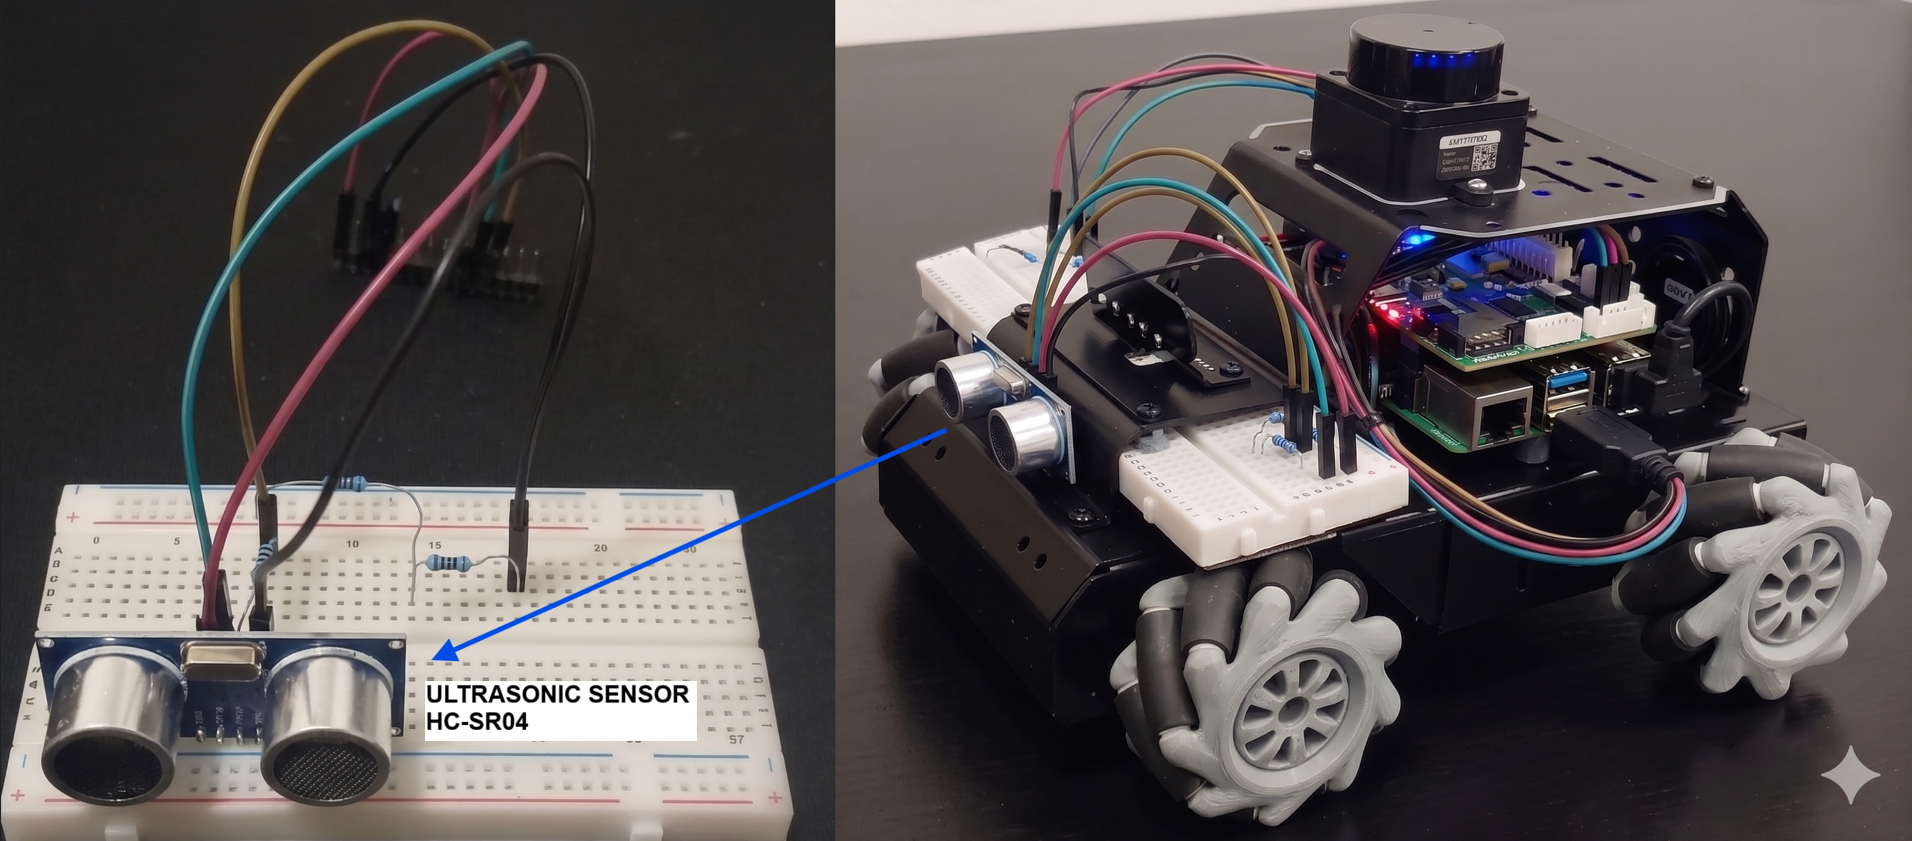
\includegraphics[width=0.48\textwidth]{ultrasonic.png}
\caption{RC Car with Ultrasonic Sensor HC-SR04}
\label{fig:pipeline}
\end{figure}

\section{Results}
The current phase of the SmartCam project has successfully transitioned from the baseline leader-follower architecture into the formalized design and component validation of a centralized, multi-agent autonomous system. The primary results of this period include finalized architectural blueprints, validated communication topologies, and integrated algorithmic pipelines engineered for deployment across the Rice University campus.

\subsection{Network Communication}
A critical bottleneck identified in early iterations was the inability of the standard ROS 2 Data Distribution Service (DDS) to operate on the university's restricted, multicast-blocking wireless network. As a result, a novel communication architecture was designed and validated. The system now uses a Tailscale Virtual Private Network (VPN) overlay in combination with the Zenoh protocol. This configuration successfully bridges ROS 2 nodes using highly compressed, unicast point-to-point connections.

\subsection{SLAM and Sensor Fusion Baseline}
Initial testing has thus far focused on establishing a stable data pipeline and characterizing raw sensor noise. To improve the robustness and accuracy of mapping, we integrate LiDAR and encoder data via a sensor-fusion pipeline. This design helps compensate for the limitations of individual sensors, such as LiDAR sparsity and noise in dynamic environments. While full-scale mapping is currently underway, SLAM was incrementally validated across two sensor configurations. The figure compares the occupancy grid maps produced by LiDAR-only versus LiDAR + Wheel Encoder. The fused configuration, however, has to be further tweaked for accuracy. Table~\ref{tab:slam} summarizes the preliminary performance metrics. The next step is to further tweak the wheel encoder data for maximum accuracy and incrementally fuse IMU data into the SLAM Toolbox backend. This will involve tuning the Kalman Filter to establish a reliable odometric baseline. Following this, the depth camera will be integrated to provide visual landmark constraints. The final validation of this phase will produce a comparative performance table quantifying RMSE for each sensor configuration. 

\begin{table}[H]
\centering
\caption{Sensor Fusion Configuration Comparison (Preliminary)}
\label{tab:slam}
\begin{tabular}{lccc}
\toprule
\textbf{Configuration} & \textbf{System Load} & \textbf{CPU (\%)} & \textbf{Latency (ms)} \\
\midrule
LiDAR             & 0.63 & 94.6 & 210 \\
LiDAR + Encoder        & 1.24 & 55.3 & 1600-4700 \\
\bottomrule
\end{tabular}
\end{table}

From the comparison results in Table~\ref{tab:slam}, the two configurations show different trade-offs between computational load and mapping latency. The LiDAR-only setup provides lower latency, while the LiDAR + Encoder setup introduces additional motion constraints that improve map consistency and reduce drift over time.
In practice, we observed that the increase in latency in the LiDAR + Encoder configuration is mainly caused by the additional processing required for sensor fusion. Unlike the LiDAR-only setup, which processes data through a relatively straightforward pipeline, the fused configuration introduces additional steps, such as encoder integration, synchronization, and filtering. These operations inevitably add computational overhead and increase the overall system delay.

Another important factor is the mismatch in update rates between different sensors. LiDAR data is typically more stable and consistent, whereas encoder readings can fluctuate with motion conditions. To combine these data sources, buffering and temporal alignment are required, which can further contribute to latency accumulation in the system.

Despite the higher latency, the fused configuration provides noticeable improvements in mapping quality. In our experiments, the LiDAR-only setup tends to produce slightly scattered map boundaries, especially during turns. After introducing encoder constraints, the trajectory becomes more stable, but this can create a bottleneck if not processed properly. To counteract this, further tweaking will be needed. Once done, accuracy levels should be improved, and the next steps can be taken to further improve efficiency.

Therefore, this result highlights a typical trade-off in embedded robotic systems: achieving better accuracy often comes at the cost of increased latency. In our case, the system remains within an acceptable real-time range, so the improvement in mapping stability is considered worthwhile for overall performance, especially given our end goal: creating a collaborative map.

\subsection{Automatic Emergency Braking} The AEB subsystem was validated in a controlled bench test. Data transmission from the Raspberry Pi (Debian OS) to the ROS2 middleware incurs approximately 0.1\,ms latency. Ultrasonic sensor data-collection latency is approximately 11.5\,ms, yielding an effective sensing loop rate of 15\,Hz. At this rate, the system provides adequate obstacle-avoidance response time at the RC car's operational speeds, with the median filter successfully suppressing spurious echo returns in the lab environment.

\subsection{YOLOv8n Object Detection} The TensorRT-optimized FP16 YOLOv8n model successfully detects people and everyday objects in real time on the Jetson Nano edge GPU. Confidence scores are consistent across standard test scenarios (e.g., cell phone at 0.90, person at 0.40 in low-light conditions). Detected bounding boxes are successfully correlated with the RealSense depth map, and the resulting 3D obstacle coordinates are injected into the ROS2 costmap, demonstrating the full perception-to-planning pipeline on embedded hardware.

\begin{table}[H]
\centering
\caption{Overall Results - SmartCam System Performance}
\label{tab:overall}
\begin{tabular}{lcc}
\toprule
\textbf{System Component} & \textbf{Latency (ms)} & \textbf{Frequency / Frame Rate} \\
\midrule
Wireless Communication & 500 & N/A \\
SLAM Mapping           & 210 & 7-15 Hz \\
AEB                    & 12  & 15 Hz \\
YOLOv8                 & N/A & 20 fps \\
\bottomrule
\end{tabular}
\end{table}

From Table~\ref{tab:overall}, we can see that different components in the system operate at very different time scales. Wireless communication introduces the highest latency, around 500 ms, which becomes one of the main bottlenecks in the overall pipeline. Compared to local processing modules, this delay is significantly larger and directly affects how quickly information can be shared between devices.

In contrast, the SLAM module maintains moderate latency while operating at a reasonable 7-15 Hz. This indicates that the mapping process is relatively stable, though it remains limited by computational cost and sensor processing. The performance is sufficient for incremental map building, but may become a constraint in more dynamic environments.

The AEB module shows much lower latency, around 12 ms, and operates at a stable frequency. This behavior is expected since AEB is designed as a safety-critical component, where fast response is prioritized over computational complexity. Its low latency ensures the system reacts quickly to nearby obstacles, even when other modules experience delays.

In the perception module, YOLOv8 achieves around 20 fps, providing a good balance between detection accuracy and real-time performance. Although it does not directly compete with AEB's latency, it is fast enough to support continuous object detection and integration into the navigation pipeline.

Overall, this table highlights an imbalance across different parts of the system. While perception and control-related modules can run efficiently on embedded hardware, communication remains the dominant source of delay. This suggests that future improvements should focus more on reducing communication overhead and optimizing data transmission, rather than only improving individual module performance.

\subsection{Centralized map merging architecture}
To achieve multi-agent environmental awareness without exceeding the computational limits of the embedded hardware, a 2D pose-graph map-merging strategy is formalized. Rather than attempting to transmit bandwidth-heavy 3D point clouds, the edge rovers utilize local SLAM algorithms to generate highly compressed 2D occupancy grids and serialized odometry graphs. The computational load of map merging will be offloaded to a central Jetson Orin Nano hub. This central server is tasked with applying graph-based backend optimization to detect geometric overlaps, establish inter-robot constraints, and elastically deform the independent local graphs into a single, unified global coordinate frame for campus-wide path planning.

\section{Discussion}
SmartCam demonstrates that a low-cost, heterogeneous edge-compute architecture can sustain a full autonomy pipeline---including SLAM, semantic perception, and emergency braking---without requiring expensive LiDAR rigs or cloud offloading. The transition from a tightly coupled socket architecture to a scalable ROS2 publish-subscribe model resolved the primary network communication bottleneck imposed by the university's restricted wireless infrastructure and positioned the system to scale to additional rover units with minimal reconfiguration.
 
The incremental sensor-fusion results confirm that adding wheel-encoder odometry to a LiDAR-only SLAM baseline meaningfully reduces boundary scatter in the occupancy grid. Quantitative RMSE comparison across all four sensor configurations remains the key next step to rigorously validate these qualitative improvements and determine the marginal accuracy gain from each added modality.
 
The AEB system's 11.5\,ms sensor loop and 0.1\,ms ROS2 handoff latency achieve a 15\,Hz safety check rate, sufficient for the RC car's current operational envelope. At higher speeds this rate may become a bottleneck, motivating a future hardware-interrupt-driven architecture for sub-millisecond response. The YOLOv8n results confirm the viability of edge inference for semantic costmap injection, though tighter RealSense-to-LiDAR temporal synchronization will be needed before field deployment.
 
Three priorities constitute the primary future work: (i) integrating IMU data into the GTSAM pose graph to further reduce rotation drift; (ii) completing the multi-agent map merging pipeline so two cars can produce a globally consistent real-time map; and (iii) deploying the full YOLOv8n depth-fusion pipeline on the physical RC car chassis for end-to-end campus field validation.

\section*{Credit Author Statement}
\small
All authors contributed equally as collaborators and shared responsibility throughout the project.  
Each author played a primary role while also supporting other aspects of the work as part of a horizontal and cooperative team effort.

\begin{itemize}
    \item \textbf{Ashley Garcia:} Conceptualization, SLAM Pipeline \& GTSAM Optimization, Methodology, Sensor Fusion, Visualization, Validation, Writing : Original Draft, Cross-Team Coordination
    \item \textbf{Mehul Goel:} Software Development, Automatic Emergency Braking, Hardware Integration, Sensor Calibration, Testing, Writing : Review \& Editing  
    \item \textbf{Chenghao Xiang:} Conceptualization, YOLOv8 Implementation, Perception Pipeline, Hardware Integration, Methodology, Visualization, Cross-Team Coordination
    \item \textbf{Youjia Tong:} Software Development, Wireless Communication Validation, Experimental Investigation, Validation, Obstacle Detection Integration, Testing, Writing : Review \& Editing 
\end{itemize}

All authors participated in discussions, reviewed the manuscript, and approved the final version for publication.

\normalsize

\section*{Acknowledgment}
\small
The authors would like to express their sincere gratitude to Professors Jose Moreto, Nakul Garg, and Joseph Young for their guidance, support, and coordination throughout the capstone project. Their advice and encouragement greatly contributed to the development of this work.

\bibliographystyle{IEEEtran}
\bibliography{references}
\end{document}